% IEEE conference paper: DSCMR and CLIP4CMR on Pascal Sentence.
% Compiles with XeLaTeX (used for DSCMR_CLIP4CMR_IEEE.pdf) or pdfLaTeX (vntex/T5 for Vietnamese names).
% On Overleaf: upload this file and fig_results.pdf (made by make_figures.py),
% fig_paired.pdf and fig_per_class.pdf;
% the default compiler works.
\documentclass[conference]{IEEEtran}

\usepackage{iftex}
\ifPDFTeX
  \usepackage[utf8]{inputenc}
  \usepackage[T5,T1]{fontenc}
  \newcommand{\vn}[1]{{\fontencoding{T5}\selectfont #1}}
\else
  \usepackage{fontspec}
  \setmainfont{texgyretermes}[Extension=.otf, UprightFont=*-regular, BoldFont=*-bold,
    ItalicFont=*-italic, BoldItalicFont=*-bolditalic]
  \newcommand{\vn}[1]{#1}
\fi
\usepackage{amsmath}
\usepackage{graphicx}
\usepackage{booktabs}
\usepackage{url}
\usepackage{tikz}
\usetikzlibrary{positioning,arrows.meta,fit,calc}

\newcommand{\Asem}{A\textsubscript{sem}}
\newcommand{\Ares}{A\textsubscript{res}}

% Same layout as IEEEtran (centered small-caps sections, left italic subsections), larger and bold.
\makeatletter
\def\section{\@startsection{section}{1}{\z@}{2.2ex plus 1ex minus .5ex}{1ex plus .3ex}%
  {\normalfont\fontsize{12}{14}\selectfont\bfseries\scshape\centering}}
\def\subsection{\@startsection{subsection}{2}{\z@}{1.6ex plus .8ex minus .4ex}{.7ex plus .2ex}%
  {\normalfont\fontsize{11}{13}\selectfont\bfseries\itshape\raggedright}}
\makeatother
\makeatletter
\newcommand{\linebreakand}{\end{@IEEEauthorhalign}\hfill\mbox{}\par\mbox{}\hfill\begin{@IEEEauthorhalign}}
\makeatother

\begin{document}

\title{Stronger Visual Features, Not New Losses: Revisiting DSCMR and CLIP4CMR on Pascal Sentence with Semantic Prototypes}

\author{
\IEEEauthorblockN{\vn{Vũ Quốc Đạt}}
\IEEEauthorblockA{DE200522\\ \textit{FPT University}\\ Da Nang, Vietnam\\ qd130506@gmail.com}
\and
\IEEEauthorblockN{\vn{Mai Quốc Huy}}
\IEEEauthorblockA{DE201068\\ \textit{FPT University}\\ Da Nang, Vietnam\\ maiquochuy100506@gmail.com}
\and
\IEEEauthorblockN{\vn{Nguyễn Gia Phúc}}
\IEEEauthorblockA{DE200407\\ \textit{FPT University}\\ Da Nang, Vietnam\\ phucoik@gmail.com}
\linebreakand
\IEEEauthorblockN{\vn{Ngô Ngọc Trường Sơn}}
\IEEEauthorblockA{DE200399\\ \textit{FPT University}\\ Da Nang, Vietnam\\ truongsonks2006@gmail.com}
\and
\IEEEauthorblockN{\vn{Trần Đăng Khoa}}
\IEEEauthorblockA{DE201144\\ \textit{FPT University}\\ Da Nang, Vietnam\\ khoatran270506@gmail.com}
\and
\IEEEauthorblockN{[Supervisor name]}
\IEEEauthorblockA{Supervisor\\ \textit{FPT University}\\ Da Nang, Vietnam\\ {[email]}}
}

\maketitle

\begin{abstract}
We revisit DSCMR and CLIP4CMR on Pascal Sentence with configurations chosen by cross-validation, validation-based checkpoints, one test evaluation per round and a declared history of test-set use; the released code of both methods selects checkpoints on the test set, which inflates mAP by up to two points. Averaged over five seeds, CLIP4CMR improves from 68.17 to 76.15 mean mAP (+7.98, 95\% CI [6.3, 9.7]). The gain comes mainly from better image features: with a stronger encoder (DFN5B ViT-H/14) whose last two image blocks are fine-tuned, the \emph{original} CLIP4CMR head already reaches 75.34. Semantic prototypes from CLIP text embeddings of class prompts, with a residual adapter and per-caption training, help most when the encoder is weak: +2.58 points with RN50, but only +0.22 with frozen DFN5B and +0.82 after fine-tuning. Learnable prototypes initialized from text are no better than fixed ones. A classify-then-rank baseline built on a zero-shot classifier is strong on this single-label benchmark (71.91 with RN50, 75.07 with DFN5B), and our best model exceeds it by only about one point. For DSCMR, a supervised contrastive loss helps only image-to-text retrieval, while stronger, partially fine-tuned features give +4.36 points.
\end{abstract}

\begin{IEEEkeywords}
cross-modal retrieval, image--text retrieval, CLIP, prototype learning, supervised contrastive learning, fine-tuning, reproducibility
\end{IEEEkeywords}

\section{Introduction}
Cross-modal retrieval aims to retrieve relevant items of one modality given a query of another, for example finding sentences that describe an image (image-to-text, I2T) or images that match a sentence (text-to-image, T2I). Because images and text live in heterogeneous feature spaces, most methods learn a common representation in which semantically related samples are close. In the supervised setting, class labels define relevance and are also used as a training signal.

DSCMR~\cite{dscmr} learns modality-specific networks with a shared classifier and combines a label-space loss, a common-space discriminative loss and a modality-invariance loss. CLIP4CMR~\cite{clip4cmr} builds on frozen features of the vision--language model CLIP~\cite{clip} and studies several objectives, among which a prototype contrastive loss (PCL) performs best. Both report results on Pascal Sentence~\cite{pascal}, a small benchmark of 1,000 images in 20 classes.

While reproducing both methods we made four observations that motivate this work. First, the released code of both methods selects the best epoch by evaluating on the test set, which yields optimistic numbers. Second, the class prototypes of CLIP4CMR are random vectors that are never trained, so they carry no semantic information although CLIP can provide it for free. Third, CLIP4CMR concatenates the five captions of each image and truncates the result to 77 tokens, discarding part of the text. Fourth, a linear probe shows that frozen image features, rather than text features, are the main bottleneck.

Our contributions are as follows:
\begin{itemize}
\item A stricter protocol (CV for model selection, validation checkpoints, five seeds, bootstrap intervals) with a declared history of test-set use, and a quantification of the bias of test-set selection.
\item Semantic prototypes with a residual adapter for CLIP4CMR, with controls (random and learnable prototypes) and a study of how their benefit depends on the encoder.
\item Per-caption training, a comparison of stronger encoders, and partial fine-tuning on an 8\,GB GPU, together with the original head on the same fine-tuned encoder to separate encoder and method.
\item Simple baselines (zero-shot, classify-then-rank) and negative results, which put the gains in perspective.
\end{itemize}

\section{Related Work}
\textbf{Supervised cross-modal retrieval.} Early methods learn linear projections that maximize correlation between modalities, notably canonical correlation analysis~\cite{cca}. Deep methods replace them with neural networks trained with label information; ACMR~\cite{acmr} adds adversarial learning to obtain modality-invariant representations, and DSCMR~\cite{dscmr} jointly minimizes discrimination losses in a label space and a common space together with a modality-invariance term.

\textbf{Vision--language pre-training.} CLIP~\cite{clip} learns aligned image and text encoders from large-scale image--text pairs and enables zero-shot classification by embedding prompts such as ``a photo of a \{class\}''. CLIP4CMR~\cite{clip4cmr} shows that frozen CLIP features substantially improve supervised cross-modal retrieval. More recent encoders improve the data or the objective, including EVA-02~\cite{eva02}, SigLIP with a sigmoid loss~\cite{siglip} and models trained on data selected by data filtering networks (DFN)~\cite{dfn}; we use the open\_clip implementations~\cite{openclip}.

\textbf{Adapting CLIP.} CLIP-Adapter~\cite{clipadapter} trains a light residual module on frozen features, which inspires our residual adapter. CoOp~\cite{coop} learns the prompt context, and Tip-Adapter~\cite{tipadapter} builds a training-free cache classifier; both use text embeddings of class names as classifier weights, as our semantic prototypes do. For fine-tuning the encoder, LP-FT~\cite{lpft} first fits a linear head and then fine-tunes everything, WiSE-FT~\cite{wiseft} interpolates zero-shot and fine-tuned weights, and FLYP~\cite{flyp} fine-tunes with the contrastive pre-training loss using class prompts as text. These methods target few-shot or full classification and robustness. We transfer two of their ideas to supervised cross-modal \emph{retrieval}: text-initialized class embeddings as prototypes of a retrieval loss that acts on both modalities, and fine-tuning only the last image blocks under an 8\,GB memory budget. We do not use weight interpolation or prompt learning. Supervised contrastive learning (SupCon)~\cite{supcon} pulls together all samples of a class and is our candidate for the common-space loss of DSCMR.

\section{Baselines and Evaluation Protocol}

\subsection{Dataset}
Pascal Sentence~\cite{pascal} contains 1,000 images from 20 classes, 50 per class, each with five captions. CLIP4CMR uses 800 training and 200 test pairs; DSCMR uses 800 training pairs and evaluates on 100 test pairs. The data link of CLIP4CMR has expired, so we recovered its feature files from a public third-party mirror. We verified that they contain exactly 800/200 distinct images with correct labels, that the image features match our own CLIP RN50 features for 922 of 1,000 images (cosine above 0.999), and that the text features match for 938 of 1,000 samples when the authors' preprocessing rule is applied. The other 78 images (15 in the test set, spread over all 20 classes) still have cosine 0.969--0.998 with our features of the same image, whereas the most similar \emph{other} image never exceeds 0.902, so they are the same images, probably decoded or resized slightly differently. To make sure the conclusions do not depend on the mirror, we reran the RN50 baseline and \Asem+B on the same split with features we extracted ourselves: 68.05\,$\pm$\,0.33 and 70.77\,$\pm$\,0.21 (mirror: 68.17 and 70.76), a paired gain of +2.72 with all five seeds improving. DSCMR releases only VGG19~\cite{vgg} fc7 features (4,096-d), 300-d text features and labels, without image identifiers; our attempts to recover the mapping to images failed, so experiments with new encoders for DSCMR use the CLIP4CMR split.

\subsection{Baselines}
DSCMR~\cite{dscmr} maps image and text features $x$ and $y$ through modality-specific networks to common-space representations $u$ and $v$, followed by a shared linear classifier with predictions $p^u, p^v$. For a batch with one-hot labels $l$, the released code minimizes
\begin{equation}
\mathcal{L}_{\mathrm{DSCMR}} = \mathcal{L}_{\mathrm{lab}} + \alpha\,\mathcal{L}_{\mathrm{com}} + \beta\,\mathcal{L}_{\mathrm{inv}},
\end{equation}
where $\mathcal{L}_{\mathrm{lab}} = \overline{\lVert p^u - l\rVert} + \overline{\lVert p^v - l\rVert}$ is the label-space loss, $\mathcal{L}_{\mathrm{inv}} = \overline{\lVert u - v\rVert}$ is the modality-invariance loss, and the common-space loss
\begin{equation}
\mathcal{L}_{\mathrm{com}} = \sum_{(a,b)} \overline{\log\!\big(1 + e^{\Gamma^{ab}_{ij}}\big) - S_{ij}\,\Gamma^{ab}_{ij}}
\end{equation}
sums over the pairs $(a,b) \in \{(u,u),(u,v),(v,v)\}$, with $\Gamma^{ab}_{ij} = \tfrac{1}{2}\cos(a_i, b_j)$, $S_{ij} = 1$ when samples $i$ and $j$ share a class, and bars denoting batch means. The defaults are $\alpha = 0.001$ and $\beta = 0.1$.

CLIP4CMR~\cite{clip4cmr} uses frozen CLIP RN50 features (1,024-d) and a two-layer projection (1024--256--1024, GELU, dropout 0.1, L2 normalization) per modality. With prototypes $c_1, \dots, c_K$, its prototype contrastive loss (PCL) for a feature $f$ of class $y$ is
\begin{equation}
\mathcal{L}_{\mathrm{PCL}}(f, y) = -\log \frac{\exp(-\lVert f - c_y\rVert^2)}{\sum_{k=1}^{K} \exp(-\lVert f - c_k\rVert^2)},
\end{equation}
applied to the image and the text output. In the released code the prototypes are random vectors that are never updated. Retrieval uses Euclidean distance in the learned space.

\subsection{Protocol}
\label{sec:protocol}
All configurations, including hyperparameters, encoders and the number of fine-tuned blocks, are selected by stratified 3-fold cross-validation (CV) on the 800 training pairs. For confirmation, each configuration is trained with five seeds (42--46) on a fixed 720/80 train/validation split, with the checkpoint chosen by validation mAP and early stopping. The test set is evaluated once, after all runs have finished. The metric is mAP over the whole retrieval set (mAP@ALL), where items sharing the class label are relevant. For a query $q$ with $R_q$ relevant items in a gallery of size $G$,
\begin{equation}
\mathrm{AP}(q) = \frac{1}{R_q} \sum_{k=1}^{G} P_q(k)\,\mathrm{rel}_q(k),
\end{equation}
where $P_q(k)$ is the precision among the top $k$ results and $\mathrm{rel}_q(k) \in \{0, 1\}$ marks a relevant item at rank $k$; mAP@ALL averages AP over all queries. Improvements are reported as paired differences against a baseline retrained with the same code, split, seeds and batch order. Standard deviations are sample standard deviations over the five seeds; 95\% confidence intervals come from 10,000 bootstrap resamples of the 200 test items (both directions of an item resampled together, per-query AP averaged over seeds).

\textbf{History of test-set use.} The protocol is applied within each round, but the study ran in rounds and later rounds were planned after seeing earlier test results, so we declare them. (i)~DSCMR loss variants with default weights, DSCMR split: test opened once. (ii)~Re-tuning of the same variants by CV, decided after (i) showed no gain: opened once. (iii)~CLIP4CMR A and B with RN50 and ViT-L/14, first on our own random split and then on the CLIP4CMR split; A, B and the CV grid for $\alpha$ were fixed before either test, which was opened once per split, and the reproduction with test-set selection (Table~\ref{tab:repro}) used the same split. (iv)~Stronger encoders and fine-tuning for both heads: \emph{this direction was chosen after (iii) showed that A+B adds only 0.30 points with ViT-L/14}, together with a train-only linear probe. All choices of the round (encoder, $N$, primary DSCMR configuration) were made by CV and fixed in a configuration file before the test was opened once. (v)~The analyses added in this revision (Table~\ref{tab:baselines}, learnable prototypes and the DFN5B column of Table~\ref{tab:ablation}, the original head with fine-tuning, the bootstrap intervals and the feature check) evaluate the CLIP4CMR test set again but select nothing. In total the CLIP4CMR test set was opened in rounds (iii), (iv) and (v), and the decisions to change the encoder and to fine-tune were taken after seeing test results of (iii).

\subsection{Reproduction}
Table~\ref{tab:repro} compares published numbers with our reproductions. Following the original code (test-set selection), CLIP4CMR is within 0.6 points of the paper and DSCMR within 1--2 points. Under our protocol both drop by about one further point, and for DSCMR test-set selection accounts for roughly two points in total. All results below use our protocol unless stated otherwise.

\begin{table}[t]
\centering
\caption{Reproduction of baselines (mAP@ALL, \%, I2T / T2I)}
\label{tab:repro}
\small
\setlength{\tabcolsep}{5pt}
\begin{tabular*}{\columnwidth}{@{\extracolsep{\fill}}lccc@{}}
\toprule
Method & Published & Test-selected & Our protocol \\
\midrule
CLIP4CMR & 69.8 / 69.2 & 69.23 / 68.95 & 68.48 / 67.87 \\
DSCMR & 71.0 / 72.2 & 68.84 / 71.05 & 66.77 / 69.32 \\
\bottomrule
\end{tabular*}

\vspace{2pt}
\parbox{\columnwidth}{\footnotesize CLIP4CMR: CLIP RN50 features, 200 test pairs. DSCMR: VGG19 features, 100 test pairs; 3 seeds under our protocol. Test-selected: best epoch chosen on the test set, as in the released code.}
\end{table}

The same comparison explains the remaining gap for DSCMR. Training exactly as in its released code for 500 epochs but reporting the \emph{last} epoch instead of the best test epoch gives only 64.22 / 67.26, so the choice of checkpoint alone moves its result by about four points.

\subsection{Implementation Details}
All experiments run on a single laptop GPU (NVIDIA RTX 5070, 8\,GB) with PyTorch 2.7.1 and deterministic algorithms enabled. Heads on frozen features follow the original optimizers (Adam, learning rate $10^{-4}$, $\beta = (0.5, 0.999)$, batch 300 for CLIP4CMR), with at most 500 epochs and early stopping after 50 epochs without improvement on the validation split. A confirmation run takes on average 31\,s for the RN50 CLIP4CMR head, 53\,s with frozen DFN5B features, 128\,s for the DSCMR head on RN50 features and 98\,s for the three-encoder ensemble. Encoder features are extracted once in fp16 and cached, so every configuration of the study can be trained on the same hardware.

\section{Proposed Improvements}

Fig.~\ref{fig:method} summarizes the four changes made to CLIP4CMR: semantic prototypes with a residual adapter (A), per-caption training (B), a stronger encoder (C) and partial fine-tuning of its image tower (D). Changes C and D are also applied to the original DSCMR head.

\begin{figure}[t]
\centering
\begin{tikzpicture}[font=\scriptsize, >={Stealth[length=1.6mm]},
  box/.style={draw, rounded corners=1.5pt, minimum height=5.2mm, align=center, inner sep=2pt},
  frz/.style={box, fill=gray!12}, trn/.style={box, fill=blue!10}, new/.style={box, fill=orange!18}]
\node[frz] (img) {Image};
\node[frz, right=3.5mm of img] (enc) {DFN5B blocks\\$1..L{-}N$ (frozen)};
\node[new, right=3.5mm of enc] (tail) {last $N$ blocks\\(fine-tuned, D)};
\node[trn, right=3.5mm of tail] (ai) {residual adapter\\(Eq.~\ref{eq:adapter})};
\node[frz, below=5mm of img] (cap) {5 captions};
\node[frz, below=5mm of enc] (tenc) {text encoder\\(frozen)};
\node[new, below=5mm of tail] (pc) {one caption / epoch\\mean at test (B)};
\node[trn, right=3.5mm of pc] (at) {adapter\\(text)};
\node[new, below=4.5mm of pc, xshift=-9mm] (proto) {class prototypes $c_k$ = text embedding of\\``a photo of a $\langle$class$\rangle$'' (A)};
\node[box] (loss) at (at |- proto) {$\mathcal{L}_{\mathrm{PCL}}$};
\draw[->] (img) -- (enc); \draw[->] (enc) -- (tail); \draw[->] (tail) -- (ai);
\draw[->] (cap) -- (tenc); \draw[->] (tenc) -- (pc); \draw[->] (pc) -- (at);
\draw[->] (ai.east) -- ++(2.5mm,0) |- (loss.east);
\draw[->] (at.south) -- (loss.north);
\draw[->] (proto) -- (loss);
\node[frz, minimum width=3mm, minimum height=2.2mm, anchor=north west] (k1) at ($(cap.south west)+(0,-14mm)$) {};
\node[right=0.5mm of k1, font=\tiny] {frozen};
\node[trn, minimum width=3mm, minimum height=2.2mm, right=10mm of k1] (k2) {};
\node[right=0.5mm of k2, font=\tiny] {trained};
\node[new, minimum width=3mm, minimum height=2.2mm, right=11mm of k2] (k3) {};
\node[right=0.5mm of k3, font=\tiny] {changed (A--D)};
\end{tikzpicture}
\caption{Improved CLIP4CMR. Encoder C is DFN5B ViT-H/14; the original method uses frozen CLIP RN50 features, concatenated captions and random fixed prototypes.}
\label{fig:method}
\end{figure}

\subsection{Semantic Prototypes with a Residual Adapter (A)}
In CLIP4CMR the prototype of each class is a random vector with gradients disabled. We instead set the prototype of class $c$ to the CLIP text embedding of the prompt ``a photo of a $\langle$class name$\rangle$'', so that semantically similar classes have nearby prototypes. To keep the pre-trained geometry while allowing adaptation, the projection of each modality is a residual adapter that mixes the frozen feature with a learned correction,
\begin{equation}
z = \mathcal{N}\big((1-\alpha)\,\mathcal{N}(x) + \alpha\,\mathcal{N}(g(x))\big),
\label{eq:adapter}
\end{equation}
where $\mathcal{N}(\cdot)$ denotes L2 normalization, $x$ is the frozen feature, $g$ is the original two-layer CLIP4CMR projection with its output dimension set to that of $x$, and $\alpha$ is chosen by CV from $\{0.1, 0.3, 0.5\}$. $\alpha = 0.3$ is best for RN50 and ViT-L/14 and within 0.05 points of the best for every other encoder, so it is used throughout. We denote this variant \Asem. As a control, \Ares{} uses the same adapter but keeps random prototypes; any gain of \Asem{} over \Ares{} can therefore be attributed to the semantics of the prototypes.

\subsection{Per-Caption Training (B)}
Instead of concatenating and truncating the five captions, we encode each caption separately. During training, one caption per image is sampled at every epoch, which acts as data augmentation; at evaluation time the text representation is the mean of the five caption embeddings.

\subsection{Stronger Encoders (C)}
A linear probe on frozen CLIP features reaches only about 73--75\% classification accuracy on images versus 77--78\% on text, indicating that the visual representation limits retrieval. We therefore extract frozen features with four larger encoders: OpenAI ViT-L/14-336, EVA02-L/14-336~\cite{eva02}, SigLIP-SO400M/14-384~\cite{siglip} and DFN5B ViT-H/14~\cite{dfn}.

\subsection{Partial Fine-Tuning (D)}
We fine-tune the last $N$ transformer blocks of the DFN5B image tower, together with its final normalization and projection, jointly with the retrieval head; the text tower stays frozen. Since earlier blocks are frozen, their output tokens are computed once and cached (recomputed features match the originals with cosine at least 0.9999996). We use learning rates of $10^{-5}$ for the encoder blocks and $10^{-4}$ for the head, Adam with $\beta = (0.5, 0.999)$, at most 100 epochs and early stopping after 20. To fit into about 3.4\,GB of free memory on an 8\,GB GPU, we use bf16, gradient checkpointing~\cite{checkpointing} and forward passes in chunks of 25 samples, which does not change the loss. $N$ is selected by CV.

\subsection{Supervised Contrastive Common-Space Loss for DSCMR}
With its default weight of 0.001, the common-space loss of DSCMR accounts for only about 0.3--1\% of the total loss, so modifying it has almost no effect. We replace it with SupCon~\cite{supcon},
\begin{equation}
\mathcal{L}_{\mathrm{SC}} = \sum_{i} \frac{-1}{|P(i)|} \sum_{p \in P(i)} \log \frac{\exp(z_i^{\top} z_p / \tau)}{\sum_{a \neq i} \exp(z_i^{\top} z_a / \tau)},
\end{equation}
computed over the normalized image and text representations $z$ of a batch, where $P(i)$ contains all other samples of the class of $i$ and $\tau = 0.2$. Separately, we test adaptive loss weights that rescale each term by the exponential moving average of its relative decrease. All loss weights are re-tuned by CV with the same budget for the baseline and the new variants. Table~\ref{tab:share} shows that tuning makes the common-space term matter: its share grows to about 3\% for the original loss and 27\% for SupCon.

\begin{table}[t]
\centering
\caption{Share of each DSCMR loss term (\%, mean up to the best epoch)}
\label{tab:share}
\small
\setlength{\tabcolsep}{4.5pt}
\begin{tabular*}{\columnwidth}{@{\extracolsep{\fill}}lccc@{}}
\toprule
Variant (tuned weights) & Label space & Common space & Invariance \\
\midrule
B0*: original loss & 86.8 & 2.8 & 10.4 \\
B1*: SupCon & 65.0 & 27.1 & 7.9 \\
B2*: adaptive weights & 86.5 & 3.0 & 10.5 \\
B3*: both & 65.4 & 26.6 & 8.0 \\
\bottomrule
\end{tabular*}

\vspace{2pt}
\parbox{\columnwidth}{\footnotesize With the default weights ($\alpha = 0.001$) the common-space share is only about 0.3--1\%. Seed 42.}
\end{table}

For DSCMR on new features, we keep its original head and loss and only change the inputs: image features from the CLIP-family encoders and the caption-mean text representation, with class-balanced batches of five samples per class. We consider an ensemble of L2-normalized DFN5B, EVA02-L and SigLIP features, concatenated and divided by $\sqrt{3}$, and DFN5B with partial fine-tuning.

\section{Experiments}

\subsection{Ablation of A and B, Fixed and Learnable Prototypes}
Table~\ref{tab:ablation} reports the ablation on the CLIP4CMR split for three frozen encoders, from weak to strong. With RN50, semantic prototypes improve both directions on every seed (+1.96), whereas the control \Ares{} is within noise of the baseline; per-caption training adds a smaller complementary gain, and \Asem+B improves by 2.58 points (5/5 seeds, 95\% CI [1.53, 3.67]). With test-set selection, as in the original paper, it reaches 71.14 / 71.00, above the published 69.8 / 69.2 with the same encoder. The benefit shrinks as the encoder gets stronger: +0.30 with ViT-L/14 and +0.22 with DFN5B, where \Asem{} alone does not help. With ViT-L/14 the adapter with random prototypes even loses 2.8 points, so an adapter without semantic prototypes is harmful.

\textbf{Learnable prototypes.} In the variant \Asem$^{\mathrm{L}}$ the prototypes are initialized from the class prompts but updated with the adapter. They move clearly (cosine 0.78--0.83 to their initialization after training) but do not help: $-$0.04 and $-$0.23 points with RN50 (without / with B, 1/5 seeds better) and $-$0.23 and +0.10 with DFN5B. The useful part of A is therefore the text initialization, not the freedom to adapt the class centers on 720 training pairs.

\begin{table}[t]
\centering
\caption{Ablation on CLIP4CMR (test, mean mAP of I2T and T2I, \%, 5 seeds)}
\label{tab:ablation}
\small
\setlength{\tabcolsep}{3pt}
\begin{tabular*}{\columnwidth}{@{\extracolsep{\fill}}lccc@{}}
\toprule
Variant & RN50 & ViT-L/14 & DFN5B \\
\midrule
Baseline & 68.17 & 71.91 & 73.40 \\
+ B & 68.80 & 72.69 & -- \\
+ \Ares{} (random prototypes) & 68.41 & 69.11 & -- \\
+ \Asem{} (fixed prototypes) & 70.13 & 72.17 & 73.25 \\
+ \Asem$^{\mathrm{L}}$ (learnable prototypes) & 70.10 & -- & 73.02 \\
\textbf{+ \Asem{} + B} & \textbf{70.76} & \textbf{72.21} & \textbf{73.62} \\
+ \Asem$^{\mathrm{L}}$ + B & 70.52 & -- & 73.72 \\
\midrule
Gain of \Asem{} + B & +2.58 (5/5) & +0.30 & +0.22 (4/5) \\
\bottomrule
\end{tabular*}

\vspace{2pt}
\parbox{\columnwidth}{\footnotesize Frozen features. Gain: paired difference to the baseline, with the number of seeds that improve. --: not run.}
\end{table}

\subsection{Encoder Comparison}
Table~\ref{tab:encoders} compares encoders by CV. Stronger encoders raise the baseline by up to about four points, and \Asem+B improves over the baseline head for every encoder (+1.0 to +2.4). DFN5B gives the best baseline and is used for fine-tuning; EVA02-L gives the best frozen \Asem+B score.

\begin{table}[t]
\centering
\caption{Encoder comparison (CV mAP, \%, average of I2T and T2I)}
\label{tab:encoders}
\small
\begin{tabular*}{\columnwidth}{@{\extracolsep{\fill}}lccc@{}}
\toprule
Encoder & Dim. & Baseline & \Asem{} + B \\
\midrule
CLIP RN50 & 1024 & 66.60 & 68.99 \\
CLIP ViT-L/14 & 768 & 68.78 & 70.79 \\
CLIP ViT-L/14-336 & 768 & 68.90 & 70.99 \\
EVA02-L/14-336 & 768 & 69.90 & 71.90 \\
SigLIP-SO400M/14-384 & 1152 & 70.21 & 71.20 \\
DFN5B ViT-H/14 & 1024 & 70.43 & 71.53 \\
\bottomrule
\end{tabular*}

\vspace{2pt}
\parbox{\columnwidth}{\footnotesize Stratified 3-fold CV on the 800 training pairs only.}
\end{table}

\subsection{Text Representation and Zero-Shot Reference}
Table~\ref{tab:text} isolates the text side. Without any training, CLIP already retrieves well above chance, and averaging the embeddings of the individual captions is clearly better than encoding their truncated concatenation (+3.4 points for RN50, +3.7 for ViT-L/14). The same holds for the DSCMR head on RN50 features (+0.9 on CV), which motivated the caption-mean input used for DSCMR throughout. With DFN5B features both text inputs perform the same, consistent with the image side being the bottleneck.

\begin{table}[t]
\centering
\caption{Text representation (mAP, \%, average of I2T and T2I)}
\label{tab:text}
\small
\begin{tabular*}{\columnwidth}{@{\extracolsep{\fill}}llcc@{}}
\toprule
Setting & Features & Concatenated & Caption mean \\
\midrule
Zero-shot CLIP (test) & RN50 & 55.15 & 58.54 \\
Zero-shot CLIP (test) & ViT-L/14 & 53.92 & 57.60 \\
DSCMR head (CV) & RN50 & 67.35 & 68.21 \\
DSCMR head (CV) & DFN5B & 72.27 & 72.24 \\
\bottomrule
\end{tabular*}

\vspace{2pt}
\parbox{\columnwidth}{\footnotesize Concatenated: five captions joined and truncated to 77 tokens, as in the original CLIP4CMR code.}
\end{table}

\subsection{Depth of Fine-Tuning}
Table~\ref{tab:depth} selects the number of fine-tuned image blocks. Fine-tuning helps both heads compared with frozen DFN5B features, by 1.7 points for CLIP4CMR and 0.8 for DSCMR on CV. Two blocks are best for CLIP4CMR, while the DSCMR head, which has more trainable parameters of its own and no semantic prototypes, profits from four.

\begin{table}[t]
\centering
\caption{Fine-tuned DFN5B image blocks (CV mAP, \%)}
\label{tab:depth}
\small
\begin{tabular*}{\columnwidth}{@{\extracolsep{\fill}}lccc@{}}
\toprule
Head & Frozen & $N = 2$ & $N = 4$ \\
\midrule
CLIP4CMR + A + B & 71.53 & \textbf{73.24} & 72.90 \\
DSCMR (original head and loss) & 72.24 & 72.71 & \textbf{73.04} \\
\bottomrule
\end{tabular*}
\end{table}

\subsection{Main Results for CLIP4CMR: Encoder versus Method}
Table~\ref{tab:clip4cmr} and Fig.~\ref{fig:results}(a) show the cumulative effect. On top of \Asem+B, frozen DFN5B features add 2.86 points and fine-tuning the last two blocks another 2.54 (CI [1.75, 3.33]; CV: 73.24 for $N = 2$, 72.90 for $N = 4$). The final model reaches 76.63 / 75.68, a paired gain of +8.15 / +7.81 over the baseline on all five seeds in both directions (each seed gains 6.4--8.9 points), about 6.5 points above the published results.

The order of this progression hides where the gain comes from. Fine-tuning the same two DFN5B blocks with the \emph{original} CLIP4CMR head (random fixed prototypes, concatenated captions, same budget and selection) already gives 75.34, i.e.\ +7.16 over the RN50 baseline (CI [5.60, 8.85]). Adding A+B to the fine-tuned encoder adds only +0.82 (+0.86 / +0.77, 5 and 4 of 5 seeds), and the interval [$-$0.26, 1.88] includes zero. About 90\% of the total gain is therefore due to the image features, and A+B matters mainly when the features are weak (Table~\ref{tab:ablation}).

\begin{table}[t]
\centering
\caption{CLIP4CMR: encoder and method (test, mAP, \%, 5 seeds)}
\label{tab:clip4cmr}
\small
\setlength{\tabcolsep}{3pt}
\begin{tabular*}{\columnwidth}{@{\extracolsep{\fill}}lcccc@{}}
\toprule
Configuration & I2T & T2I & Avg. & 95\% CI \\
\midrule
Baseline (RN50) & 68.48 & 67.87 & 68.17 & [63.9, 72.3] \\
+ \Asem{} + B (RN50) & 70.90 & 70.61 & 70.76 & [66.9, 74.5] \\
+ DFN5B (frozen) & 73.71 & 73.53 & 73.62 & [69.9, 77.2] \\
DFN5B FT 2 bl., original head & 75.77 & 74.91 & 75.34 & [71.4, 79.2] \\
\textbf{DFN5B FT 2 bl. + \Asem{} + B} & \textbf{76.63} & \textbf{75.68} & \textbf{76.15} & [72.5, 79.6] \\
\bottomrule
\end{tabular*}

\vspace{2pt}
\parbox{\columnwidth}{\footnotesize Seed standard deviations are 0.2--0.7. CI: bootstrap over the 200 test items; paired intervals of differences are given in the text and are much narrower.}
\end{table}

\begin{figure}[t]
\centering
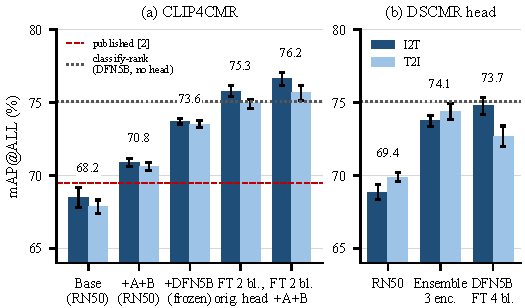
\includegraphics[width=\columnwidth]{fig_results.pdf}
\caption{Test mAP@ALL (\%, mean and sample standard deviation over 5 seeds) for (a) CLIP4CMR improvements and (b) the original DSCMR head on different input features. Numbers above bars are the average of both directions; the dashed line marks the published result of CLIP4CMR~\cite{clip4cmr}, the dotted line the classify-then-rank baseline with DFN5B (no retrieval head).}
\label{fig:results}
\end{figure}

\begin{figure}[t]
\centering
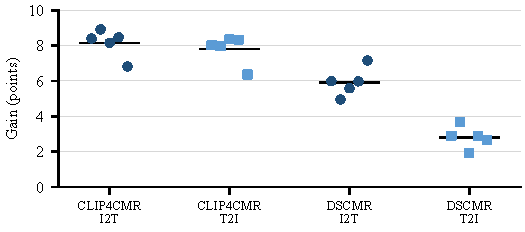
\includegraphics[width=\columnwidth]{fig_paired.pdf}
\caption{Paired gain of the final models over their RN50 baselines for each seed (markers) and on average (horizontal lines). All 20 gains are positive.}
\label{fig:paired}
\end{figure}

Fig.~\ref{fig:paired} shows that the improvement does not depend on a lucky seed: each of the five seeds gains between 6.4 and 8.9 points for CLIP4CMR in both directions, roughly ten times the seed-to-seed standard deviation in Table~\ref{tab:clip4cmr}. For DSCMR every seed also improves, by 4.9--7.2 points for I2T and by a smaller 1.9--3.7 points for T2I.

\subsection{Simple Baselines}
Because relevance is defined by a single class label, retrieval on Pascal Sentence is closely tied to classification. Table~\ref{tab:baselines} therefore reports baselines without any retrieval head. Zero-shot retrieval compares image and text embeddings directly; averaging the caption embeddings beats the truncated concatenation by 2--3 points, which motivates B. \emph{Classify-then-rank} predicts class probabilities $p$ for every image and text, either with a zero-shot classifier (softmax over cosine similarities to the class prompts, temperature 0.01) or with a logistic-regression probe per modality trained on the 800 training pairs (regularization chosen by CV), and ranks by $p_{\mathrm{img}}^{\top} p_{\mathrm{txt}}$.

\begin{table}[t]
\centering
\caption{Baselines without a retrieval head (test, mean mAP of I2T and T2I, \%)}
\label{tab:baselines}
\small
\setlength{\tabcolsep}{4pt}
\begin{tabular*}{\columnwidth}{@{\extracolsep{\fill}}lccc@{}}
\toprule
Method (frozen features) & RN50 & DFN5B & Acc. (DFN5B) \\
\midrule
Zero-shot, concatenated captions & 55.15 & 58.79 & -- \\
Zero-shot, caption mean & 58.54 & 61.06 & -- \\
Classify-then-rank, zero-shot clf. & 71.91 & 75.07 & 83.5 / 78.5 \\
Classify-then-rank, linear probe & 69.96 & 75.12 & 82.5 / 82.5 \\
\bottomrule
\end{tabular*}

\vspace{2pt}
\parbox{\columnwidth}{\footnotesize Deterministic (no seeds). Acc.: test classification accuracy for images / texts. Classify-then-rank scores a pair by the inner product of the predicted class distributions.}
\end{table}

The classify-then-rank baselines are strong. With RN50 features the zero-shot variant (71.91) beats the trained CLIP4CMR baseline by 3.7 points (95\% CI [1.6, 5.8]) and is level with \Asem+B ($-$1.2, CI [$-$2.9, 0.6]). With DFN5B features it reaches 75.07, above frozen \Asem+B (73.62) and the fine-tuned DSCMR head (73.74); the final CLIP4CMR model is ahead by only 1.09 points (CI [$-$0.30, 2.53]), and by 1.03 (CI [$-$0.21, 2.30]) over the probe. On this benchmark the trained heads therefore add little beyond a good zero-shot classifier, and their advantage comes mostly from the image features. This also explains why semantic prototypes help: they inject the zero-shot classifier into the retrieval loss. For classification, the RN50 zero-shot classifier is right for 78.0\% of images and texts and the probe for 76.0\% / 83.0\%. The nearest-prototype accuracy of the final model is 85.3\% for images and 79.7\% for texts, against 82.3\% / 81.4\% with frozen DFN5B: fine-tuning improves the image side only.

\subsection{Results for DSCMR}
Table~\ref{tab:dscmrloss} shows the loss modifications on the original DSCMR split and features. SupCon improves I2T by 1.15 points on all five seeds but does not improve T2I, and none of the tuned variants exceeds the default-weight baseline (68.05 average over three seeds). Adaptive loss weights have almost no effect.

\begin{table}[t]
\centering
\caption{Loss modifications for DSCMR (original split, test, 5 seeds)}
\label{tab:dscmrloss}
\small
\begin{tabular*}{\columnwidth}{@{\extracolsep{\fill}}lccc@{}}
\toprule
Variant (tuned weights) & I2T & T2I & Paired gain (seeds) \\
\midrule
B0*: original loss & 66.02 & 68.42 & -- \\
B1*: SupCon, $\tau = 0.2$ & 67.17 & 68.24 & +1.15 / $-$0.18 (5, 1) \\
B2*: adaptive weights & 66.52 & 68.40 & +0.50 / $-$0.02 (4, 2) \\
B3*: both & 67.06 & 68.07 & +1.04 / $-$0.35 (5, 3) \\
\bottomrule
\end{tabular*}

\vspace{2pt}
\parbox{\columnwidth}{\footnotesize Reference: DSCMR with default weights reaches 66.77 / 69.32 (3 seeds).}
\end{table}

Table~\ref{tab:dscmrfeat} and Fig.~\ref{fig:results}(b) report the original DSCMR head on the CLIP4CMR split with new input features. Using caption-mean RN50 features gives a baseline of 69.38. DFN5B features raise the CV score by about four points, and the two candidate configurations are virtually tied on CV (73.04 for fine-tuning four blocks, 73.03 for the ensemble; two blocks give 72.71). Following the rule fixed before opening the test set, the fine-tuned model is the primary configuration. It improves by +4.36 on average (+5.93 / +2.81 paired, 5/5 seeds); the ensemble, reported as secondary, reaches 74.06.

\begin{table}[t]
\centering
\caption{Original DSCMR head on new features (test, 5 seeds)}
\label{tab:dscmrfeat}
\small
\setlength{\tabcolsep}{4pt}
\begin{tabular*}{\columnwidth}{@{\extracolsep{\fill}}lccc@{}}
\toprule
Input features & I2T & T2I & Avg. \\
\midrule
RN50 (baseline) & 68.86 $\pm$ 0.53 & 69.89 $\pm$ 0.31 & 69.38 \\
3-encoder ensemble$^\dagger$ & 73.75 $\pm$ 0.37 & 74.38 $\pm$ 0.53 & 74.06 \\
\textbf{DFN5B, FT 4 blocks} & \textbf{74.78 $\pm$ 0.57} & \textbf{72.70 $\pm$ 0.69} & \textbf{73.74} \\
\bottomrule
\end{tabular*}

\vspace{2pt}
\parbox{\columnwidth}{\footnotesize CLIP4CMR split; text features are the mean of the five caption embeddings. Bold: primary configuration, fixed before opening the test set. $^\dagger$Secondary configuration.}
\end{table}

\subsection{Per-Class Analysis}
Fig.~\ref{fig:perclass} breaks the CLIP4CMR result down by class. Animals and vehicles with a distinctive appearance (sheep, train, cow, horse, cat) are retrieved almost perfectly by both models. The hardest classes are person, potted plant and chair: their images are often cluttered indoor or street scenes in which the labeled object is small and appears together with objects of other classes, so the captions may describe something else. The improved model gains much on these ambiguous classes (person +14.9, chair +15.6) and most on sofa (+37.0, from 47.6 to 84.6), a class whose indoor scenes overlap with chair and dining table.

\begin{figure}[t]
\centering
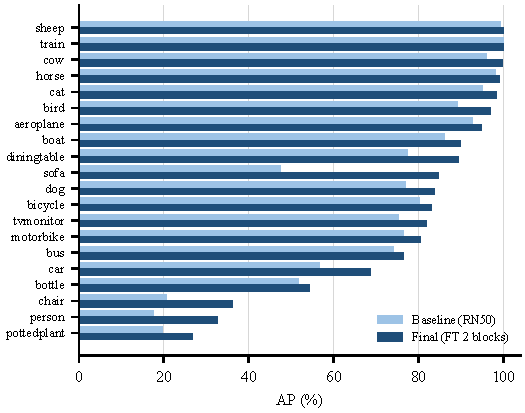
\includegraphics[width=\columnwidth]{fig_per_class.pdf}
\caption{Average precision per class for CLIP4CMR (mean over 5 seeds and both directions), sorted by the final model.}
\label{fig:perclass}
\end{figure}

\section{Discussion}
\textbf{Sources of improvement.} For CLIP4CMR, most of the gain comes from the image encoder: the original head on the fine-tuned DFN5B encoder recovers 7.16 of the 7.98 points. Semantic prototypes are worth +2.6 points with RN50 but at most about 0.8 with strong features, and making them learnable does not help. The control experiment is important: an adapter with random prototypes does not help and can hurt, so the gain of A comes from injecting class semantics. Their effect is best understood through the classify-then-rank baseline: on a single-label benchmark retrieval is close to classification, and text prototypes give the head a zero-shot classifier for free, which matters when the head cannot learn a good one from weak features. For DSCMR, almost the entire gain also comes from better input features: strengthening its nearly inactive common-space term improved only one retrieval direction.

\textbf{Negative results.} Beyond the DSCMR loss variants, we tested post-hoc re-ranking with dual-softmax normalization and database-side augmentation (Table~\ref{tab:rerank}). The best setting helps CLIP4CMR with \Asem+B on RN50 features (+0.89 on CV), but only +0.15 with DFN5B features, and it hurts the baseline head and the DSCMR head. Since it also requires access to the whole retrieval set at query time, it was not used. Fine-tuning more blocks did not help CLIP4CMR (4 blocks: 72.90 versus 73.24 on CV).

\begin{table}[t]
\centering
\caption{Post-hoc re-ranking (CV mAP, \%, average of both directions)}
\label{tab:rerank}
\small
\begin{tabular*}{\columnwidth}{@{\extracolsep{\fill}}llccc@{}}
\toprule
Features & Head & None & Dual-softmax & $\Delta$ \\
\midrule
RN50 & CLIP4CMR & 66.60 & 66.21 & $-$0.39 \\
RN50 & CLIP4CMR + A + B & 68.99 & 69.88 & +0.89 \\
RN50 & DSCMR & 68.21 & 67.56 & $-$0.64 \\
DFN5B & CLIP4CMR & 70.43 & 70.08 & $-$0.35 \\
DFN5B & CLIP4CMR + A + B & 71.53 & 71.68 & +0.15 \\
DFN5B & DSCMR & 72.24 & 71.42 & $-$0.81 \\
\bottomrule
\end{tabular*}

\vspace{2pt}
\parbox{\columnwidth}{\footnotesize Best re-ranking setting per row (dual-softmax, $\tau = 0.1$); database-side augmentation was never the best setting.}
\end{table}

\textbf{Reproducibility.} The repository provides every script, the saved predictions and logs of all runs, the trained weights of all five seeds as release assets, and a notebook that recomputes every reported test number from the saved test embeddings without a GPU. The tag \texttt{experiments-2026-10-31} marks the exact code version that produced the original results; the analyses added in this revision are in \texttt{reports/revision\_20261112}.

\textbf{Limitations.} The CLIP4CMR split comes from a third-party mirror that, although verified, has not been confirmed by the authors. The improved DSCMR is evaluated on the CLIP4CMR split and therefore cannot be compared with its published numbers on the same test set. Most of the improvement is due to a stronger pre-trained encoder, which also requires more computation, and a training-free classify-then-rank baseline is within about one point of our best model. The test set was reused across rounds (Section~\ref{sec:protocol}). All results are on a single small dataset with 200 test pairs; a second benchmark such as Wikipedia or NUS-WIDE is left for future work.

\section{Conclusion}
We revisited DSCMR and CLIP4CMR under a protocol that does not use the test set for model selection. CLIP4CMR improves from 68.17 to 76.15 mean mAP on Pascal Sentence, consistently across seeds, but the gain comes mainly from better image features: the original head on a partially fine-tuned DFN5B encoder reaches 75.34. Semantic prototypes from class prompts help most when the encoder is weak (+2.6 points with RN50), and a zero-shot classify-then-rank baseline is within about one point of the best model. For DSCMR, a supervised contrastive loss helps only image-to-text retrieval, while stronger features add 4.36 points. Evaluation protocol, simple baselines and the choice of encoder matter more on this benchmark than the retrieval head.

Code and results: \url{https://github.com/sotbatchien123/dscmr-clip4cmr-pascal}

\section*{Author Contributions}
\vn{Ngô Ngọc Trường Sơn}: idea, implementation, all experiments, analysis and writing. \vn{Nguyễn Gia Phúc}: unit tests of the retrieval metrics. \vn{Vũ Quốc Đạt}: verification of the references. \vn{Mai Quốc Huy}: installation check on a clean machine and the troubleshooting guide. \vn{Trần Đăng Khoa}: proofreading of the abstract and author information. All authors read and approved the paper.

\section*{Use of AI Tools}
AI assistants (Claude and Codex) were used to help write and debug code, to run and check experiments and to draft and edit the text. The authors checked every reported number against the saved outputs and take full responsibility for the code, the results and the paper.

\begin{thebibliography}{00}
\bibitem{dscmr} L. Zhen, P. Hu, X. Wang, and D. Peng, ``Deep supervised cross-modal retrieval,'' in \textit{Proc. IEEE/CVF Conf. Comput. Vis. Pattern Recognit. (CVPR)}, 2019, pp. 10394--10403.
\bibitem{clip4cmr} Z. Zeng and W. Mao, ``A comprehensive empirical study of vision-language pre-trained model for supervised cross-modal retrieval,'' arXiv:2201.02772, 2022.
\bibitem{clip} A. Radford \textit{et al.}, ``Learning transferable visual models from natural language supervision,'' in \textit{Proc. Int. Conf. Mach. Learn. (ICML)}, 2021, pp. 8748--8763.
\bibitem{pascal} C. Rashtchian, P. Young, M. Hodosh, and J. Hockenmaier, ``Collecting image annotations using Amazon's Mechanical Turk,'' in \textit{Proc. NAACL HLT Workshop Creating Speech Lang. Data Amazon's Mechanical Turk}, 2010, pp. 139--147.
\bibitem{supcon} P. Khosla \textit{et al.}, ``Supervised contrastive learning,'' in \textit{Proc. Adv. Neural Inf. Process. Syst. (NeurIPS)}, 2020.
\bibitem{dfn} A. Fang, A. M. Jose, A. Jain, L. Schmidt, A. Toshev, and V. Shankar, ``Data filtering networks,'' in \textit{Proc. Int. Conf. Learn. Represent. (ICLR)}, 2024.
\bibitem{eva02} Y. Fang, Q. Sun, X. Wang, T. Huang, X. Wang, and Y. Cao, ``EVA-02: A visual representation for neon genesis,'' arXiv:2303.11331, 2023.
\bibitem{siglip} X. Zhai, B. Mustafa, A. Kolesnikov, and L. Beyer, ``Sigmoid loss for language image pre-training,'' in \textit{Proc. IEEE/CVF Int. Conf. Comput. Vis. (ICCV)}, 2023, pp. 11975--11986.
\bibitem{checkpointing} T. Chen, B. Xu, C. Zhang, and C. Guestrin, ``Training deep nets with sublinear memory cost,'' arXiv:1604.06174, 2016.
\bibitem{clipadapter} P. Gao \textit{et al.}, ``CLIP-Adapter: Better vision-language models with feature adapters,'' \textit{Int. J. Comput. Vis.}, vol. 132, no. 2, pp. 581--595, 2024, doi: 10.1007/s11263-023-01891-x.
\bibitem{vgg} K. Simonyan and A. Zisserman, ``Very deep convolutional networks for large-scale image recognition,'' in \textit{Proc. Int. Conf. Learn. Represent. (ICLR)}, 2015.
\bibitem{openclip} G. Ilharco \textit{et al.}, ``OpenCLIP,'' Zenodo, 2021, doi: 10.5281/zenodo.5143773.
\bibitem{cca} D. R. Hardoon, S. Szedmak, and J. Shawe-Taylor, ``Canonical correlation analysis: An overview with application to learning methods,'' \textit{Neural Comput.}, vol. 16, no. 12, pp. 2639--2664, 2004, doi: 10.1162/0899766042321814.
\bibitem{acmr} B. Wang, Y. Yang, X. Xu, A. Hanjalic, and H. T. Shen, ``Adversarial cross-modal retrieval,'' in \textit{Proc. ACM Int. Conf. Multimedia}, 2017, pp. 154--162, doi: 10.1145/3123266.3123326.
\bibitem{coop} K. Zhou, J. Yang, C. C. Loy, and Z. Liu, ``Learning to prompt for vision-language models,'' \textit{Int. J. Comput. Vis.}, vol. 130, no. 9, pp. 2337--2348, 2022.
\bibitem{tipadapter} R. Zhang \textit{et al.}, ``Tip-Adapter: Training-free adaption of CLIP for few-shot classification,'' in \textit{Proc. Eur. Conf. Comput. Vis. (ECCV)}, 2022, pp. 493--510.
\bibitem{lpft} A. Kumar, A. Raghunathan, R. Jones, T. Ma, and P. Liang, ``Fine-tuning can distort pretrained features and underperform out-of-distribution,'' in \textit{Proc. Int. Conf. Learn. Represent. (ICLR)}, 2022.
\bibitem{wiseft} M. Wortsman \textit{et al.}, ``Robust fine-tuning of zero-shot models,'' in \textit{Proc. IEEE/CVF Conf. Comput. Vis. Pattern Recognit. (CVPR)}, 2022, pp. 7959--7971.
\bibitem{flyp} S. Goyal, A. Kumar, S. Garg, Z. Kolter, and A. Raghunathan, ``Finetune like you pretrain: Improved finetuning of zero-shot vision models,'' in \textit{Proc. IEEE/CVF Conf. Comput. Vis. Pattern Recognit. (CVPR)}, 2023, pp. 19338--19347.
\end{thebibliography}

\end{document}
